\usepackage[letterpaper,left=1.20in,right=1.20in,top=1.00in,bottom=1.05in,includehead,includefoot,headsep=14pt,footskip=26pt]{geometry}
\usepackage{microtype}
\usepackage{mathtools}
\usepackage{amssymb}
\usepackage{mathrsfs}
\usepackage{centernot}
\usepackage{float}
\usepackage{caption}
\usepackage{fancyhdr}
\usepackage{titlesec}
\usepackage{enumitem}
\usepackage{titling}
\usepackage[most]{tcolorbox}
\usepackage{etoolbox}
\usepackage{booktabs}
\usepackage{tabularx}
\usepackage{array}
\usepackage{pdflscape}
\usepackage{adjustbox}
\usepackage{needspace}
\usepackage{xurl}   % long URLs break at any character
\graphicspath{{src/}{./}}

\definecolor{tnnavy}{HTML}{173B5E}
\definecolor{tnblue}{HTML}{275DAD}
\definecolor{tnteal}{HTML}{2A9D8F}
\definecolor{tnrust}{HTML}{B84A2B}
\definecolor{tncream}{HTML}{F7F2E8}
\definecolor{tnlightblue}{HTML}{EDF4FA}
\definecolor{tngray}{HTML}{4B5563}


% ---- status vocabulary -------------------------------------------------
\definecolor{tngreen}{HTML}{1F7A4D}
\definecolor{tnamber}{HTML}{8A6D1F}

\newcommand{\tnstatusbox}[2]{%
  {\setlength{\fboxsep}{2.1pt}%
   \colorbox{#1}{\textcolor{white}{\scriptsize\bfseries\hspace{0.5pt}#2\hspace{0.5pt}}}}}
\newcommand{\PROVED}{\tnstatusbox{tngreen}{PROVED}}
\newcommand{\CERT}{\tnstatusbox{tnblue}{CERTIFIED}}
\newcommand{\EQUIV}{\tnstatusbox{tnnavy}{RH-EQUIVALENT}}
\newcommand{\OPENSTAT}{\tnstatusbox{tnrust}{OPEN}}
\newcommand{\EVID}{\tnstatusbox{tnamber}{EVIDENCE}}

% a figure pointer whose tie survives the markdown reader
\newcommand{\figref}[1]{Figure~\ref{#1}}

\newcommand{\statuslegend}{%
\begin{center}\small
\begin{tabular}{@{}l@{\hspace{7pt}}p{0.78\textwidth}@{}}
\PROVED{} & proved here or cited as proved: an unconditional theorem or an exact identity.\\[1.6pt]
\CERT{} & rigorous but computer-assisted, or dependent on verified zero heights; the finite region it certifies is stated with it.\\[1.6pt]
\EQUIV{} & logically equivalent to the Riemann hypothesis. An equivalence is not a proof in either direction.\\[1.6pt]
\OPENSTAT{} & not proved anywhere in this work, and not implied by any finite result in it.\\[1.6pt]
\EVID{} & numerical or empirical support only. It never upgrades a status.\\
\end{tabular}
\end{center}}

\newtcolorbox{tnclosed}[1]{enhanced,breakable,
  colback=white,colframe=tngreen,boxrule=1.1pt,arc=2pt,
  left=7pt,right=7pt,top=6pt,bottom=6pt,
  fonttitle=\bfseries\scriptsize,coltitle=white,colbacktitle=tngreen,
  title={CLOSED FORM\quad\normalfont\itshape #1}}

\newtcolorbox{tnequiv}[1]{enhanced,breakable,
  colback=tnlightblue,colframe=tnnavy,boxrule=1.1pt,arc=2pt,
  left=7pt,right=7pt,top=6pt,bottom=6pt,
  fonttitle=\bfseries\scriptsize,coltitle=white,colbacktitle=tnnavy,
  title={RH-EQUIVALENT\quad\normalfont\itshape #1}}

\newtcolorbox{tnopen}[1]{enhanced,breakable,
  colback=white,colframe=tnrust,boxrule=1.1pt,arc=2pt,
  left=7pt,right=7pt,top=6pt,bottom=6pt,
  fonttitle=\bfseries\scriptsize,coltitle=white,colbacktitle=tnrust,
  title={OPEN\quad\normalfont\itshape #1}}
% -----------------------------------------------------------------------------


% Page fill: leave slack at the foot rather than stretching every gap.
\raggedbottom
\setlength{\parskip}{3.4pt plus 1.0pt minus 0.8pt}
\AtBeginDocument{%
  \setlength{\abovedisplayskip}{6.0pt plus 1.8pt minus 2.2pt}%
  \setlength{\belowdisplayskip}{6.0pt plus 1.8pt minus 2.2pt}%
  \setlength{\abovedisplayshortskip}{2.5pt plus 1pt}%
  \setlength{\belowdisplayshortskip}{4.5pt plus 1pt}%
}

% Figures stay exactly where the text puts them. The single exception is
% the wide master grid, set [p] below, which takes a page of its own so
% that the text page before it fills instead of being abandoned.
\floatplacement{figure}{H}
% float packing
\setcounter{topnumber}{3}\setcounter{bottomnumber}{2}\setcounter{totalnumber}{5}
\renewcommand{\topfraction}{0.92}\renewcommand{\bottomfraction}{0.75}
\renewcommand{\textfraction}{0.06}
\renewcommand{\floatpagefraction}{0.78}
\DeclareCaptionFont{tnnavyfont}{\color{tnnavy}}
\DeclareCaptionFont{tngrayfont}{\color{tngray}}
\captionsetup{
  font=small,
  labelfont={bf,tnnavyfont},
  textfont=tngrayfont,
  justification=centering,
  singlelinecheck=false,
  skip=5pt
}

\setlist{itemsep=2pt,topsep=4pt}
\renewcommand{\arraystretch}{1.13}
\AtBeginEnvironment{longtable}{\scriptsize\setlength{\tabcolsep}{3pt}}
\let\cleardoublepage\clearpage

% A Part opens on a fresh page only when less than a third of the current
% page remains; otherwise it follows the previous Part's last paragraph. This
% returns the white space that chapter-style openers spent at every Part end.
\titleclass{\chapter}{straight}
\titleformat{name=\chapter,numberless}[display]
  {\Needspace*{17\baselineskip}\normalfont\huge\bfseries\color{tnnavy}}
  {}
  {0pt}
  {\titlerule[1.1pt]\vspace{0.7ex}\filright}
  [\vspace{0.6ex}\titlerule]

\titleformat{\section}
  {\normalfont\Large\bfseries\color{tnnavy}}
  {}
  {0pt}
  {}

\titleformat{\subsection}
  {\normalfont\large\bfseries\color{tnteal}}
  {}
  {0pt}
  {}

\titlespacing*{\chapter}{0pt}{26pt}{16pt}
\titlespacing*{\section}{0pt}{17pt}{7pt}
\titlespacing*{\subsection}{0pt}{12.5pt}{5pt}

\setlength{\droptitle}{-3.3em}
\pretitle{\begin{center}\color{tnnavy}\Huge\bfseries}
\posttitle{%
  \par\end{center}
  \vspace{0.35em}
  \begin{center}
    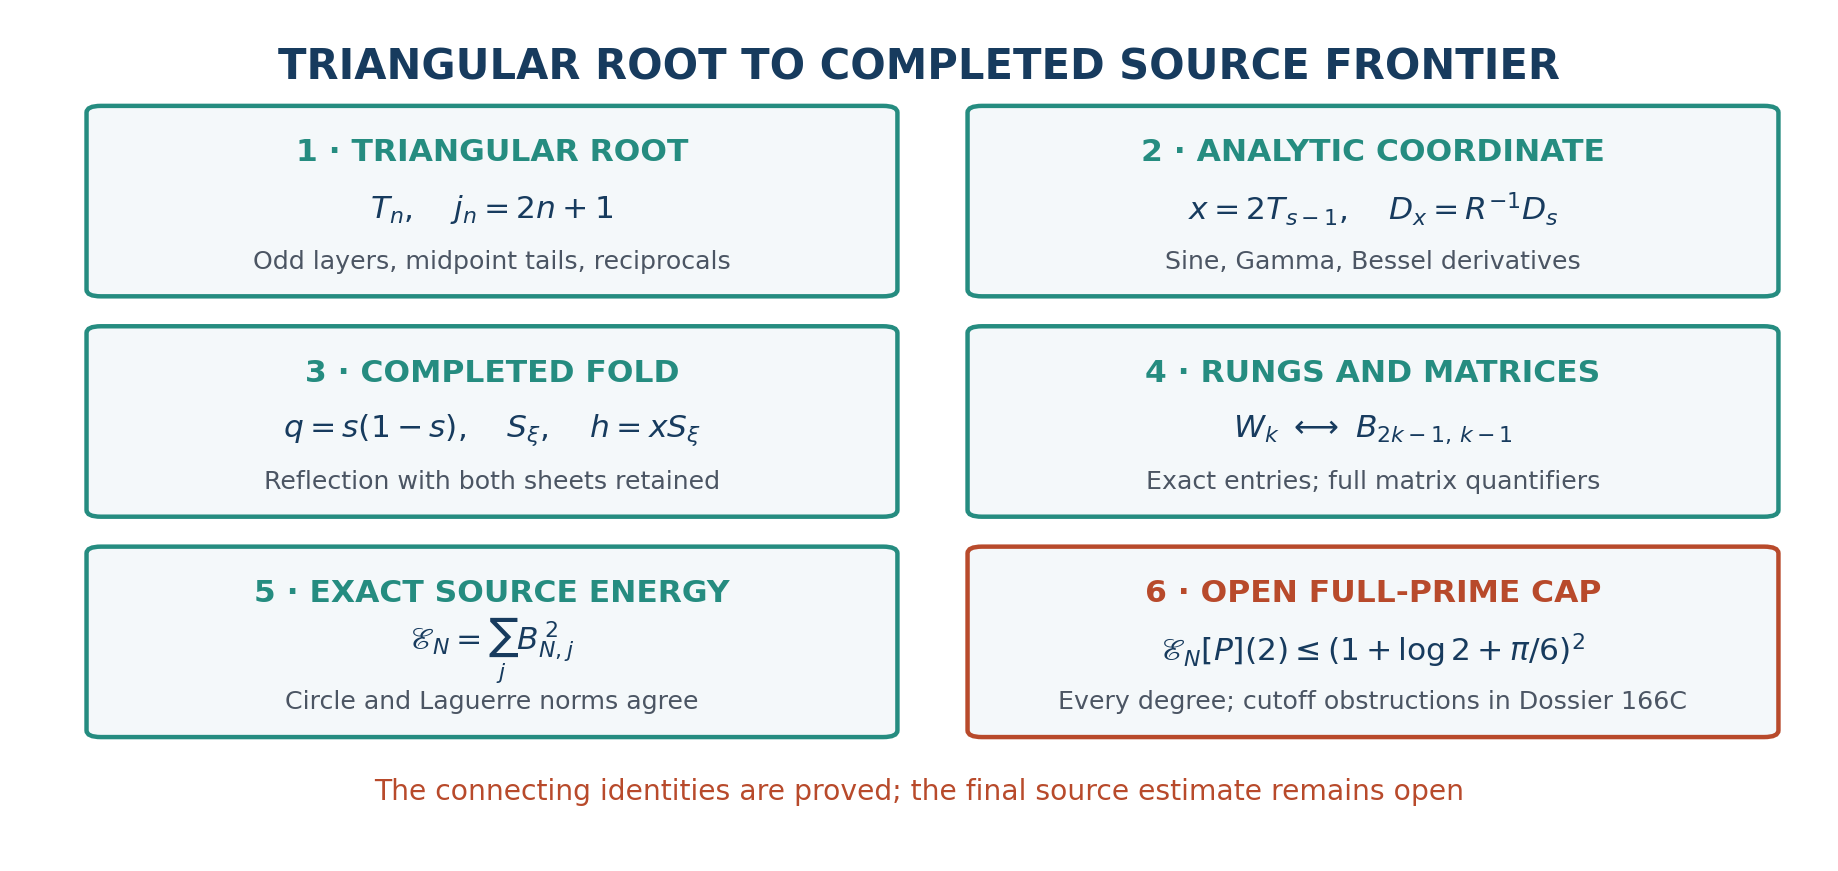
\includegraphics[width=0.96\textwidth]{figures/v32_triangular_root_map.png}
  \end{center}
  \vspace{0.25em}
}
\preauthor{\begin{center}\large\lineskip .5em\begin{tabular}[t]{c}}
\postauthor{\end{tabular}\par\end{center}}
\predate{\begin{center}\normalsize}
\postdate{%
  \par\vspace{0.35em}
  {\color{tnrust}\bfseries RH STATUS: OPEN}
  \par\end{center}\thispagestyle{empty}
}

\pagestyle{fancy}
\fancyhf{}
\fancyhead[R]{\small\color{tngray}\thepage}
\fancyhead[L]{\small\color{tngray}\nouppercase{\rightmark}}
\fancyfoot[L]{\scriptsize\color{tngray}$s=\sigma+it$}
\fancyfoot[C]{\scriptsize\color{tngray}Volume I -- Reading Volume, v5.0 -- RH OPEN}
\renewcommand{\headrulewidth}{0.4pt}
\renewcommand{\footrulewidth}{0pt}
\setlength{\headheight}{15pt}

% A two-column contents list: the same depth, a third of the pages.
\usepackage{multicol}
\makeatletter
\renewcommand{\tableofcontents}{%
  \chapter*{\contentsname}%
  \@mkboth{\contentsname}{\contentsname}%
  \begingroup\small\setlength{\columnsep}{20pt}%
  \begin{multicols}{2}\@starttoc{toc}\end{multicols}%
  \endgroup}
\makeatother

\renewenvironment{quote}
  {\begin{tcolorbox}[
      enhanced,
      breakable,
      colback=tncream,
      colframe=tnrust,
      boxrule=0.8pt,
      arc=1.5pt,
      left=7pt,
      right=7pt,
      top=6pt,
      bottom=6pt]}
  {\end{tcolorbox}}

\AtBeginDocument{
  \hypersetup{
    linkcolor=tnblue,
    urlcolor=tnteal,
    citecolor=tnrust,
    pdfauthor={Jeffery Huckstead; Cerebral Graphix},
    pdftitle={Triangular-n Postmaster: From the Discrete Primitive to the Completed Source Frontier},
    pdfsubject={v5.0 reading volume: triangular coordinates, Euler constant bridge, completed folding, Widder sectors, Li-Loewner geometry, Bernstein-Laguerre energy, exponential prime cutoffs and the open fixed-scale prime estimate; Riemann hypothesis open}
  }
}
